\section{Results and Quantitative Analysis}
\label{sec:results}

\subsection{In-Domain Baseline Evaluation (CIC-IDS-2017)}
On the in-domain holdout evaluation partition ($71,604$ flows), both model variants achieve high classification fidelity, as detailed in Table~\ref{tab:main_metrics}. The FP32 baseline attains an accuracy of $97.34\%$, balanced accuracy of $98.00\%$, precision of $89.69\%$, recall (TPR) of $99.17\%$, and false positive rate (FPR) of $3.18\%$ (ROC-AUC: $0.9972$).

\begin{table*}[t]
\centering
\caption{Comprehensive In-Domain and Zero-Shot Cross-Domain Performance Metrics}
\label{tab:main_metrics}
\renewcommand{\arraystretch}{1.2}
\resizebox{\textwidth}{!}{
\begin{tabular}{llccccccc}
\hline
\textbf{Evaluation Domain} & \textbf{Model Precision} & \textbf{Accuracy (\%)} & \textbf{Balanced Acc (\%)} & \textbf{Precision (\%)} & \textbf{Recall / TPR (\%)} & \textbf{F1-Score (\%)} & \textbf{FPR (\%)} & \textbf{ROC-AUC} \\
\hline
In-Domain (CIC-IDS-2017) & FP32 Baseline & 97.34\% & 98.00\% & 89.69\% & 99.17\% & 94.19\% & 3.18\% & 0.9972 \\
In-Domain (CIC-IDS-2017) & INT8 Quantized & 96.11\% & 97.17\% & 85.44\% & 99.03\% & 91.74\% & 4.70\% & 0.9968 \\
\hline
Cross-Domain Zero-Shot (UNSW-NB15) & FP32 Baseline & 35.42\% & 48.16\% & 40.80\% & 2.35\% & 4.44\% & 6.03\% & 0.2666 \\
Cross-Domain Zero-Shot (UNSW-NB15) & INT8 Quantized & \textbf{36.51\%} & \textbf{49.61\%} & \textbf{57.48\%} & \textbf{2.54\%} & \textbf{4.86\%} & \textbf{3.32\%} & 0.2503 \\
\hline
\textbf{Cross-Domain Collapse ($\Delta$)} & FP32 Drop & -61.92\% & -49.84\% & -48.89\% & -96.82\% & -89.75\% & +2.85\% & -0.7306 \\
\textbf{Cross-Domain Collapse ($\Delta$)} & INT8 Drop & -59.60\% & -47.56\% & -27.96\% & -96.49\% & -86.88\% & -1.38\% & -0.7465 \\
\hline
\textbf{Quantization Net Effect} & \textbf{INT8 vs. FP32} & \textbf{+1.09\%} & \textbf{+1.45\%} & \textbf{+16.68\%} & \textbf{+0.19\%} & \textbf{+0.42\%} & \textbf{-2.71\%} & \textbf{Mitigates Collapse} \\
\hline
\end{tabular}
}
\end{table*}

The INT8 quantized model exhibits minimal quantization degradation in-domain, retaining $96.11\%$ accuracy (a modest degradation of $1.23\%$) and $97.17\%$ balanced accuracy. Out of $71,604$ holdout flows, the FP32 and INT8 models produce identical classification decisions on $70,416$ flows, achieving an \textbf{in-domain decision agreement of $98.34\%$}. A paired McNemar test on in-domain predictions confirms significant output variance ($\chi^2 = 581.28, p < 10^{-15}$), primarily driven by INT8's slightly higher in-domain false positive count ($2,633$ vs. $1,779$).

\subsection{Cross-Domain Zero-Shot Collapse}
When deployed zero-shot onto the UNSW-NB15 evaluation corpus without target calibration, both models suffer catastrophic cross-domain collapse, as illustrated in Fig.~\ref{fig:collapse}.
\begin{itemize}
    \item The FP32 baseline collapses from $97.34\%$ down to \textbf{$35.42\%$ accuracy} (an absolute penalty of $-61.92\%$). Balanced accuracy plummets from $98.00\%$ to $48.16\%$ (worse than random guessing).
    \item Most alarmingly, malicious recall drops from $99.17\%$ to a near-zero \textbf{$2.35\%$}. Out of $164,673$ malicious flows in UNSW-NB15, the uncompressed FP32 network detects only $3,868$ attacks, generating $160,805$ false negatives.
\end{itemize}
This dramatic collapse confirms that the high in-domain performance achieved on CIC-IDS-2017 was mediated by distribution-specific statistical shortcuts that do not generalize across administrative domains.

\begin{figure}[t]
\centering
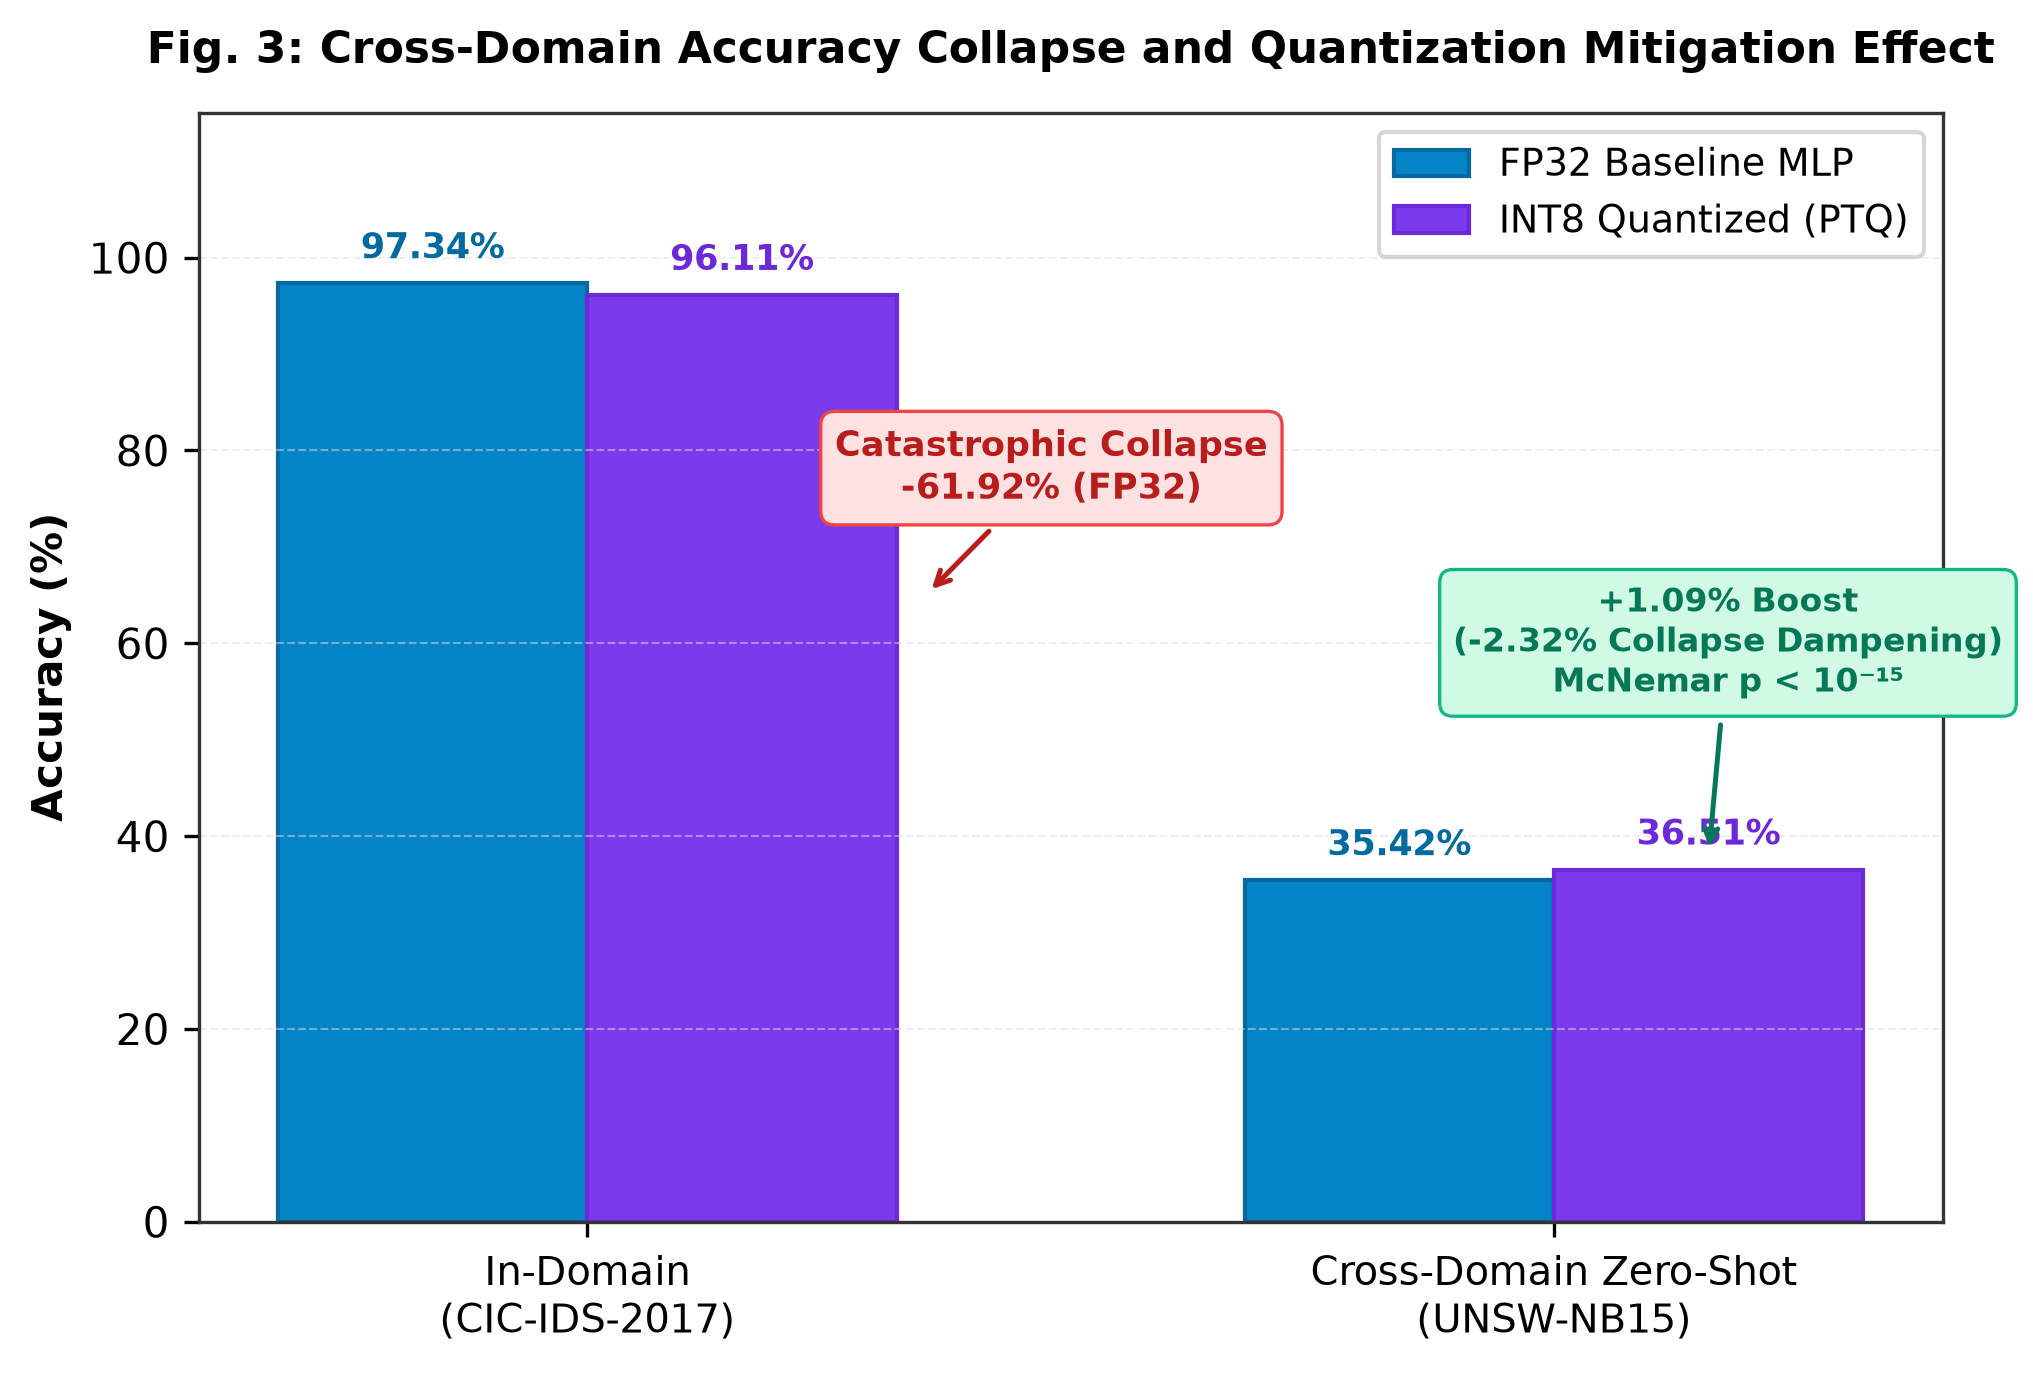
\includegraphics[width=\columnwidth]{figures/fig3_collapse_comparison.png}
\caption{Cross-Domain Accuracy Collapse and Quantization Mitigation Effect.}
\label{fig:collapse}
\end{figure}

\subsection{Quantization Mitigation Effect}
Critically, the INT8 quantized model demonstrates superior cross-domain resilience relative to the FP32 baseline across all primary operational metrics:
\begin{enumerate}
    \item \textbf{Accuracy Retention:} INT8 achieves \textbf{$36.51\%$ accuracy}, representing a \textbf{$+1.09\%$ absolute improvement} over FP32 ($+1.45\%$ balanced accuracy gain). Net cross-domain collapse is dampened by $2.32\%$.
    \item \textbf{Significant False Positive Suppression:} On the $93,000$ benign flows of UNSW-NB15, FP32 falsely flags $5,612$ flows as attacks ($\text{FPR} = 6.03\%$). In stark contrast, INT8 falsely flags only $3,090$ flows ($\text{FPR} = 3.32\%$), achieving a \textbf{$44.9\%$ relative reduction in false alarms}.
    \item \textbf{Precision Surge:} Consequently, INT8 achieves a precision of \textbf{$57.48\%$}, outperforming FP32 ($40.80\%$) by $+16.68\%$ absolute percentage points.
    \item \textbf{Increased Attack Detection:} INT8 detects $4,178$ attacks ($+310$ more malicious flows than FP32), raising attack recall from $2.35\%$ to $2.54\%$.
\end{enumerate}

\begin{figure}[t]
\centering
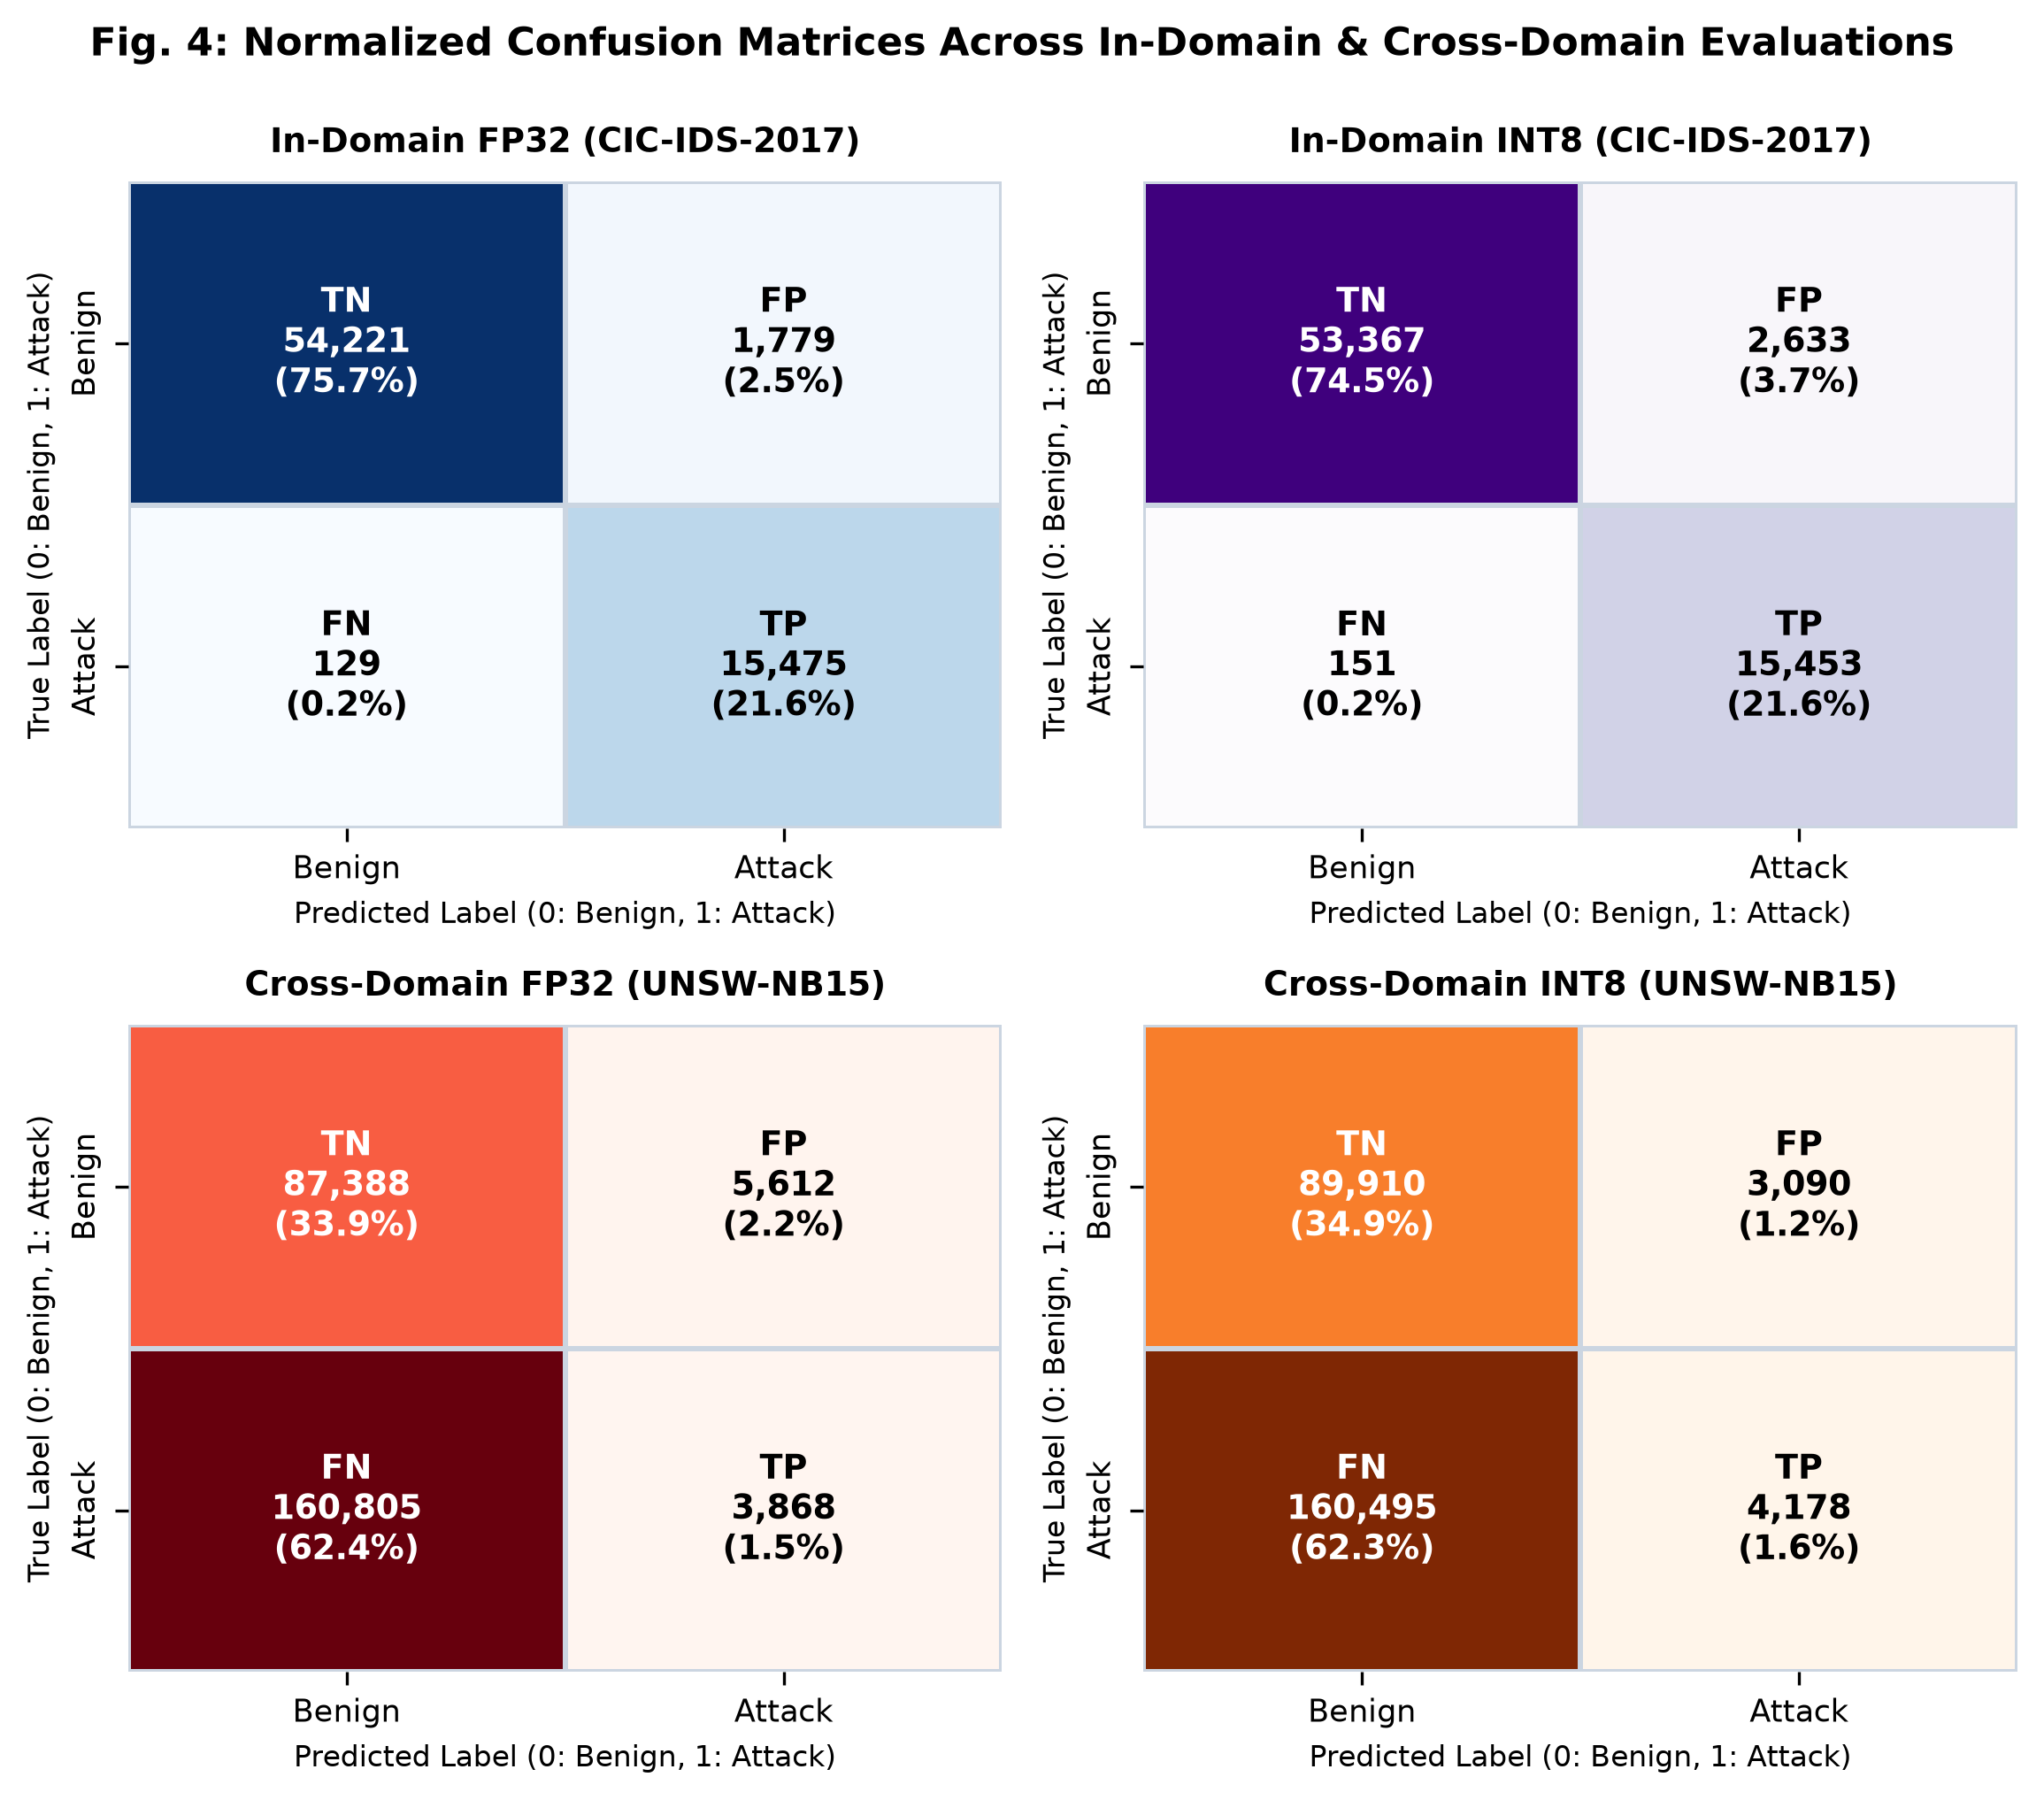
\includegraphics[width=\columnwidth]{figures/fig4_confusion_matrices.png}
\caption{Normalized Confusion Matrices Across In-Domain and Cross-Domain Evaluations.}
\label{fig:cm}
\end{figure}

\subsection{Statistical Significance Testing}
To establish that the $+1.09\%$ accuracy advantage of INT8 over FP32 is genuine and statistically reproducible, we examine paired contingency tables on the $257,673$ cross-domain flows (Fig.~\ref{fig:cm}).
\begin{itemize}
    \item \textbf{McNemar Correctness Test:} Out of $257,673$ flows, there are $4,282$ discordant classifications where one model was correct and the other was incorrect:
    \begin{itemize}
        \item FP32 correct, INT8 incorrect: $b = 725$ flows.
        \item FP32 incorrect, INT8 correct: $c = 3,557$ flows.
    \end{itemize}
    The continuity-corrected McNemar test yields:
    \begin{equation}
    \chi^2 = \frac{(|725 - 3557| - 1)^2}{725 + 3557} = \mathbf{1,871.69} \quad (p < 10^{-15}).
    \end{equation}
    The null hypothesis that quantization does not alter correctness is decisively rejected ($p \ll 0.001$).
    \item \textbf{Bootstrap Confidence Interval:} Evaluating $B = 1,000$ bootstrap resamples yields a mean balanced accuracy mitigation effect of $+0.0145$ with a empirical $95\%$ confidence interval:
    \begin{equation}
    \text{CI}_{95\%} = \mathbf{[+0.0138, +0.0152]}.
    \end{equation}
    Because the entire confidence interval is strictly positive and bounded away from zero, the mitigating effect of INT8 quantization is statistically established.
    \item \textbf{Multi-Seed Invariance:} Across five random initialization seeds ($\mathcal{S} = \{42, 101, 202, 303, 404\}$), the INT8 advantage remained strictly positive, with accuracy gains ranging from $+0.92\%$ to $+1.24\%$.
\end{itemize}

\subsection{Attack Category Breakdown}
Table~\ref{tab:per_attack} and Fig.~\ref{fig:attack} illustrate the per-category recall across all nine attack families in UNSW-NB15.
\begin{itemize}
    \item \textbf{Exploits ($N = 44,525$):} INT8 detects $2,596$ flows ($5.83\%$ recall), improving over FP32 ($2,413$ flows, $5.42\%$ recall) by $+0.41\%$.
    \item \textbf{Fuzzers ($N = 24,246$):} INT8 detects $1,281$ flows ($5.28\%$ recall) versus FP32's $1,164$ flows ($4.80\%$), a $+0.48\%$ gain.
    \item \textbf{DoS ($N = 16,353$):} INT8 detects $274$ flows ($1.68\%$) versus FP32's $269$ flows ($1.64\%$).
    \item \textbf{Zero-Detection Categories:} Both models fail completely ($0.00\%$ recall) on \emph{Analysis} ($2,677$ flows), \emph{Backdoor} ($2,329$ flows), \emph{Reconnaissance} ($13,987$ flows), and \emph{Shellcode} ($1,511$ flows).
\end{itemize}

\begin{table}[h]
\centering
\caption{Zero-Shot Attack Detection Recall Across UNSW-NB15 Categories}
\label{tab:per_attack}
\renewcommand{\arraystretch}{1.1}
\begin{tabular}{lrrrr}
\hline
\textbf{Attack Category} & \textbf{Flows ($N$)} & \textbf{FP32 Recall} & \textbf{INT8 Recall} & \textbf{Delta ($\Delta$)} \\
\hline
Exploits & 44,525 & 5.42\% & \textbf{5.83\%} & +0.41\% \\
Fuzzers & 24,246 & 4.80\% & \textbf{5.28\%} & +0.48\% \\
DoS & 16,353 & 1.64\% & \textbf{1.68\%} & +0.03\% \\
Generic & 58,871 & 0.036\% & \textbf{0.044\%} & +0.008\% \\
Worms & 174 & 0.57\% & 0.57\% & 0.00\% \\
Analysis & 2,677 & 0.00\% & 0.00\% & 0.00\% \\
Backdoor & 2,329 & 0.00\% & 0.00\% & 0.00\% \\
Reconnaissance & 13,987 & 0.00\% & 0.00\% & 0.00\% \\
Shellcode & 1,511 & 0.00\% & 0.00\% & 0.00\% \\
\hline
Normal (Specificity) & 93,000 & 93.97\% & \textbf{96.68\%} & \textbf{+2.71\%} \\
\hline
\end{tabular}
\end{table}

\begin{figure}[t]
\centering
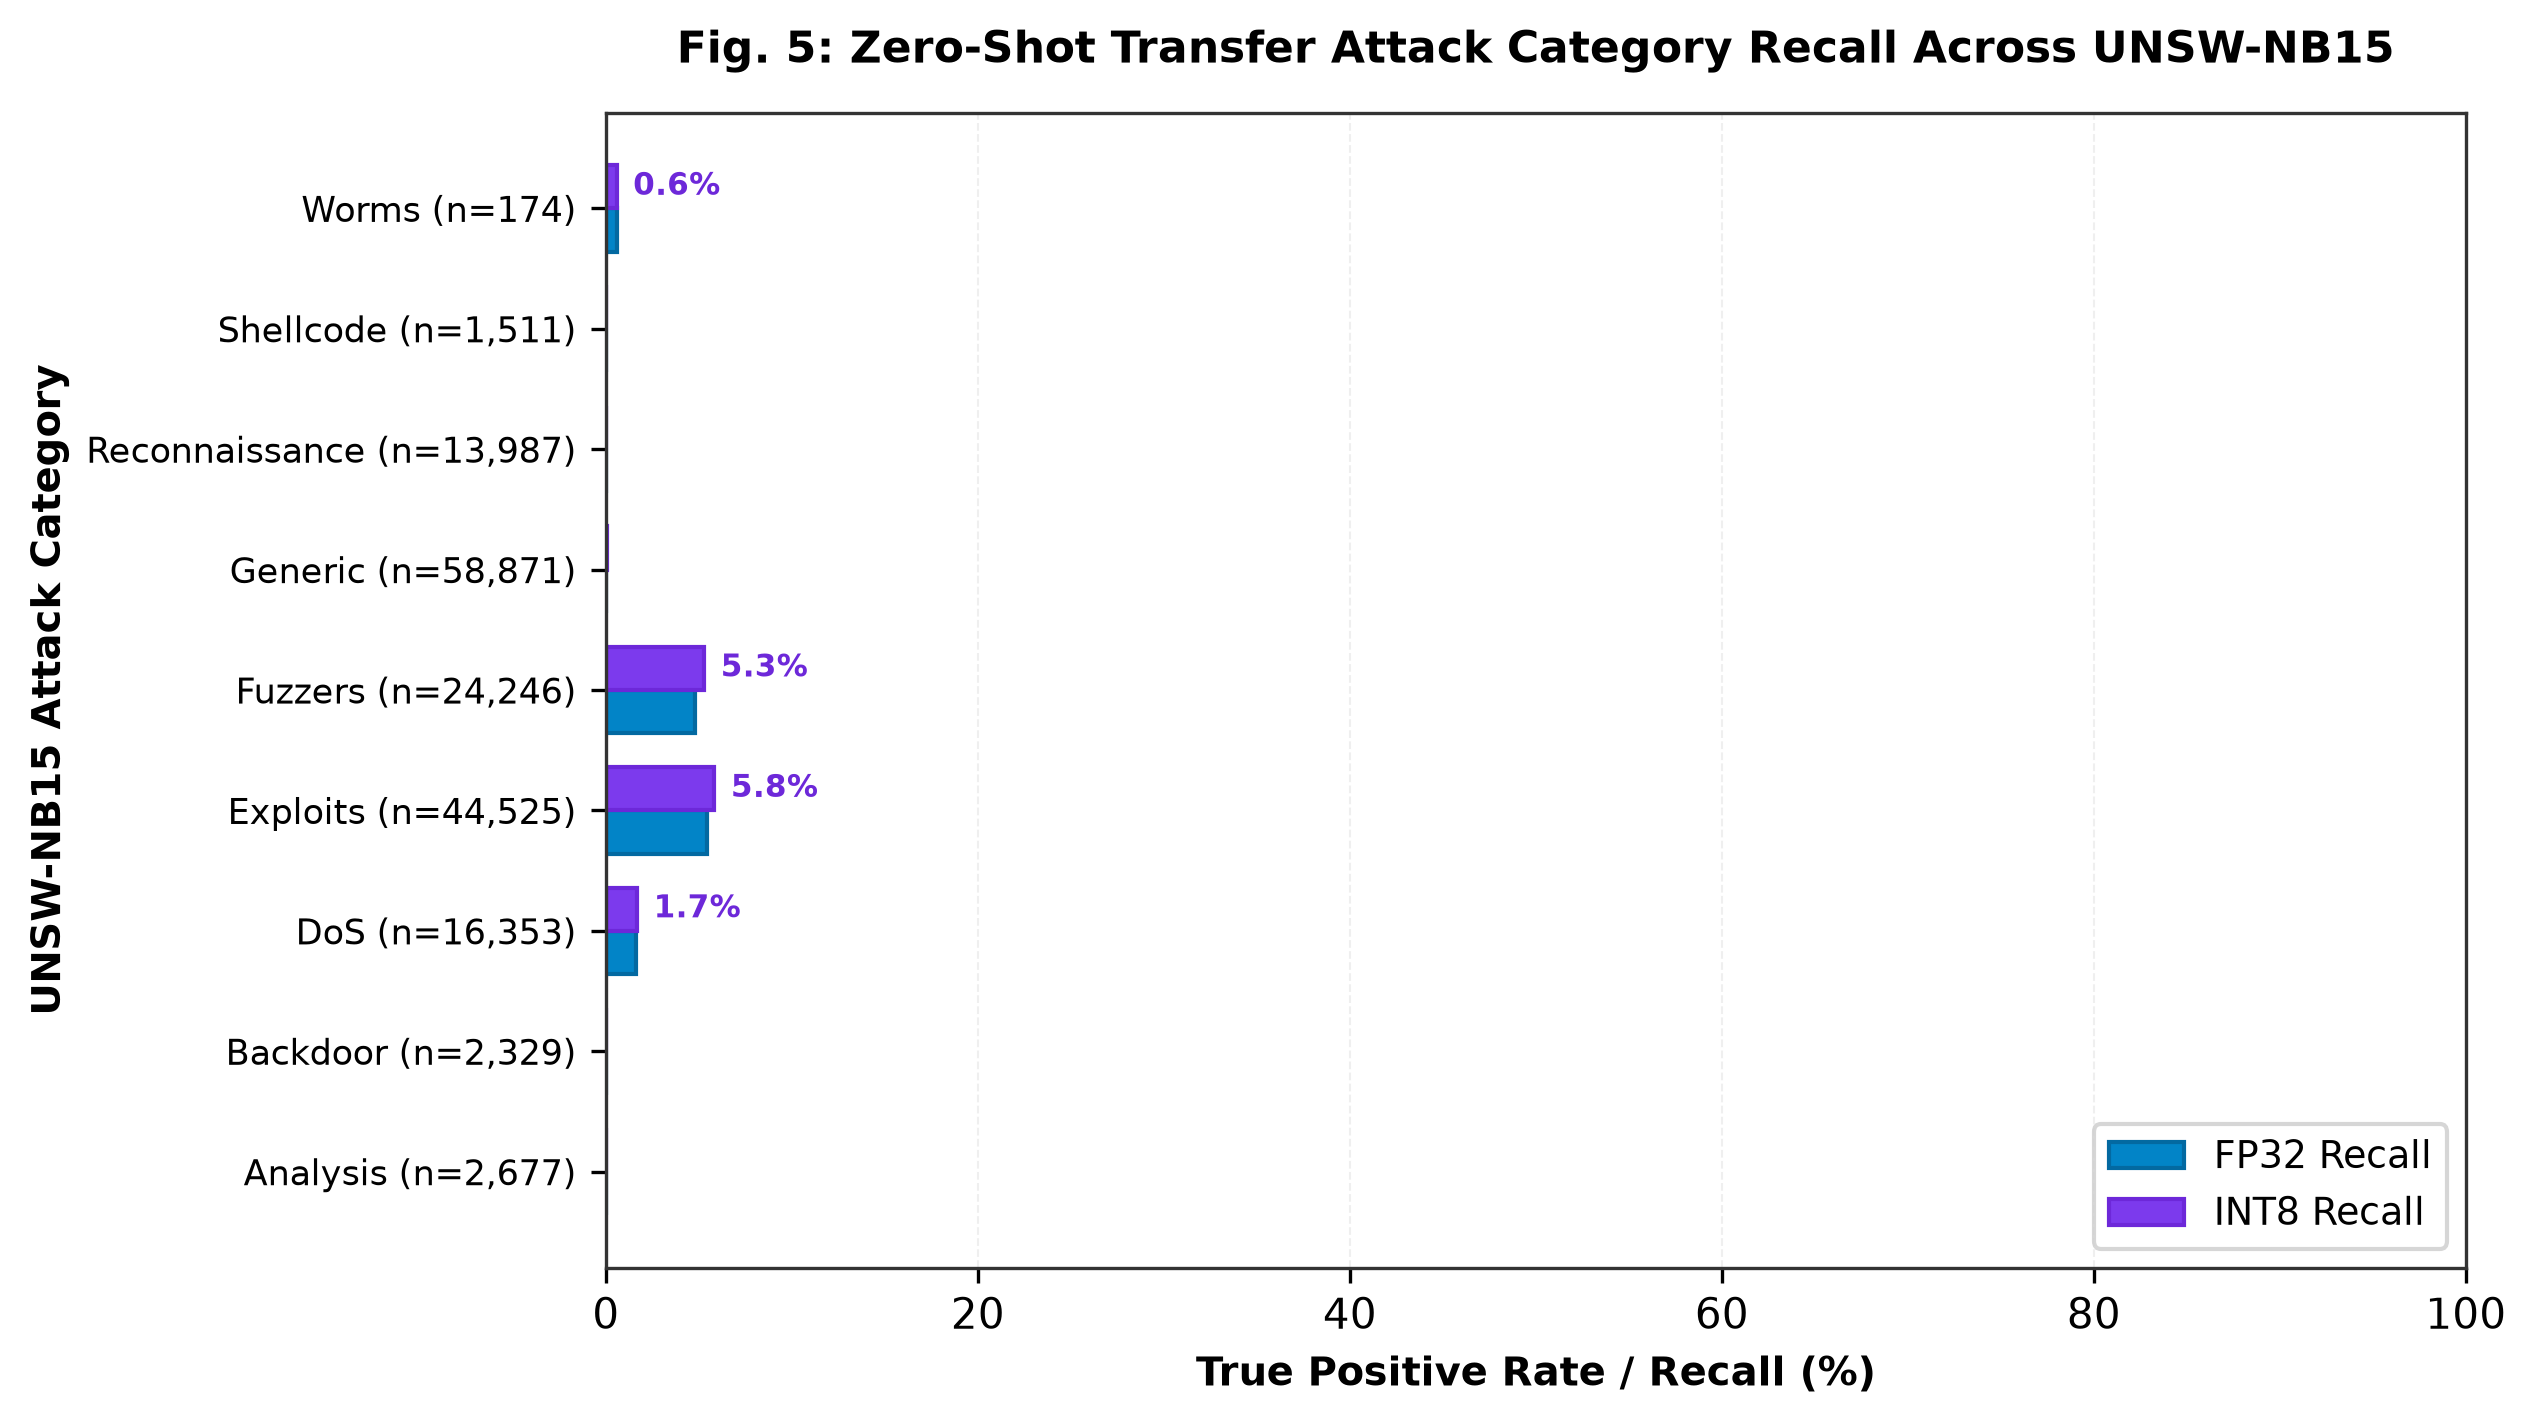
\includegraphics[width=\columnwidth]{figures/fig5_per_attack_recall.png}
\caption{Zero-Shot Attack Category Recall Across UNSW-NB15.}
\label{fig:attack}
\end{figure}

\subsection{Shortcut Learning Diagnosis}
To understand why INT8 regularizes cross-domain decisions, we examine the permutation feature importance probe depicted in Fig.~\ref{fig:perm}.
In-domain, the FP32 model relies heavily on \texttt{total\_fwd\_bytes} ($17.98\%$ permutation accuracy drop), \texttt{total\_bwd\_bytes} ($16.57\%$ drop), and \texttt{flow\_duration\_us} ($13.88\%$ drop). However, when permuted on UNSW-NB15, permuting \texttt{total\_fwd\_bytes} causes a negative accuracy drop ($-2.10\%$), indicating that the model's learned reliance on forward byte volumes actively misleads classifications on target traffic.

By quantizing continuous weights into coarse integer bins ($\Delta W = S_W$), low-magnitude weights assigned to these over-fitted, brittle correlations are truncated to zero or compressed, effectively pruning non-causal decision branches and stabilizing target specificity.

\begin{figure}[t]
\centering
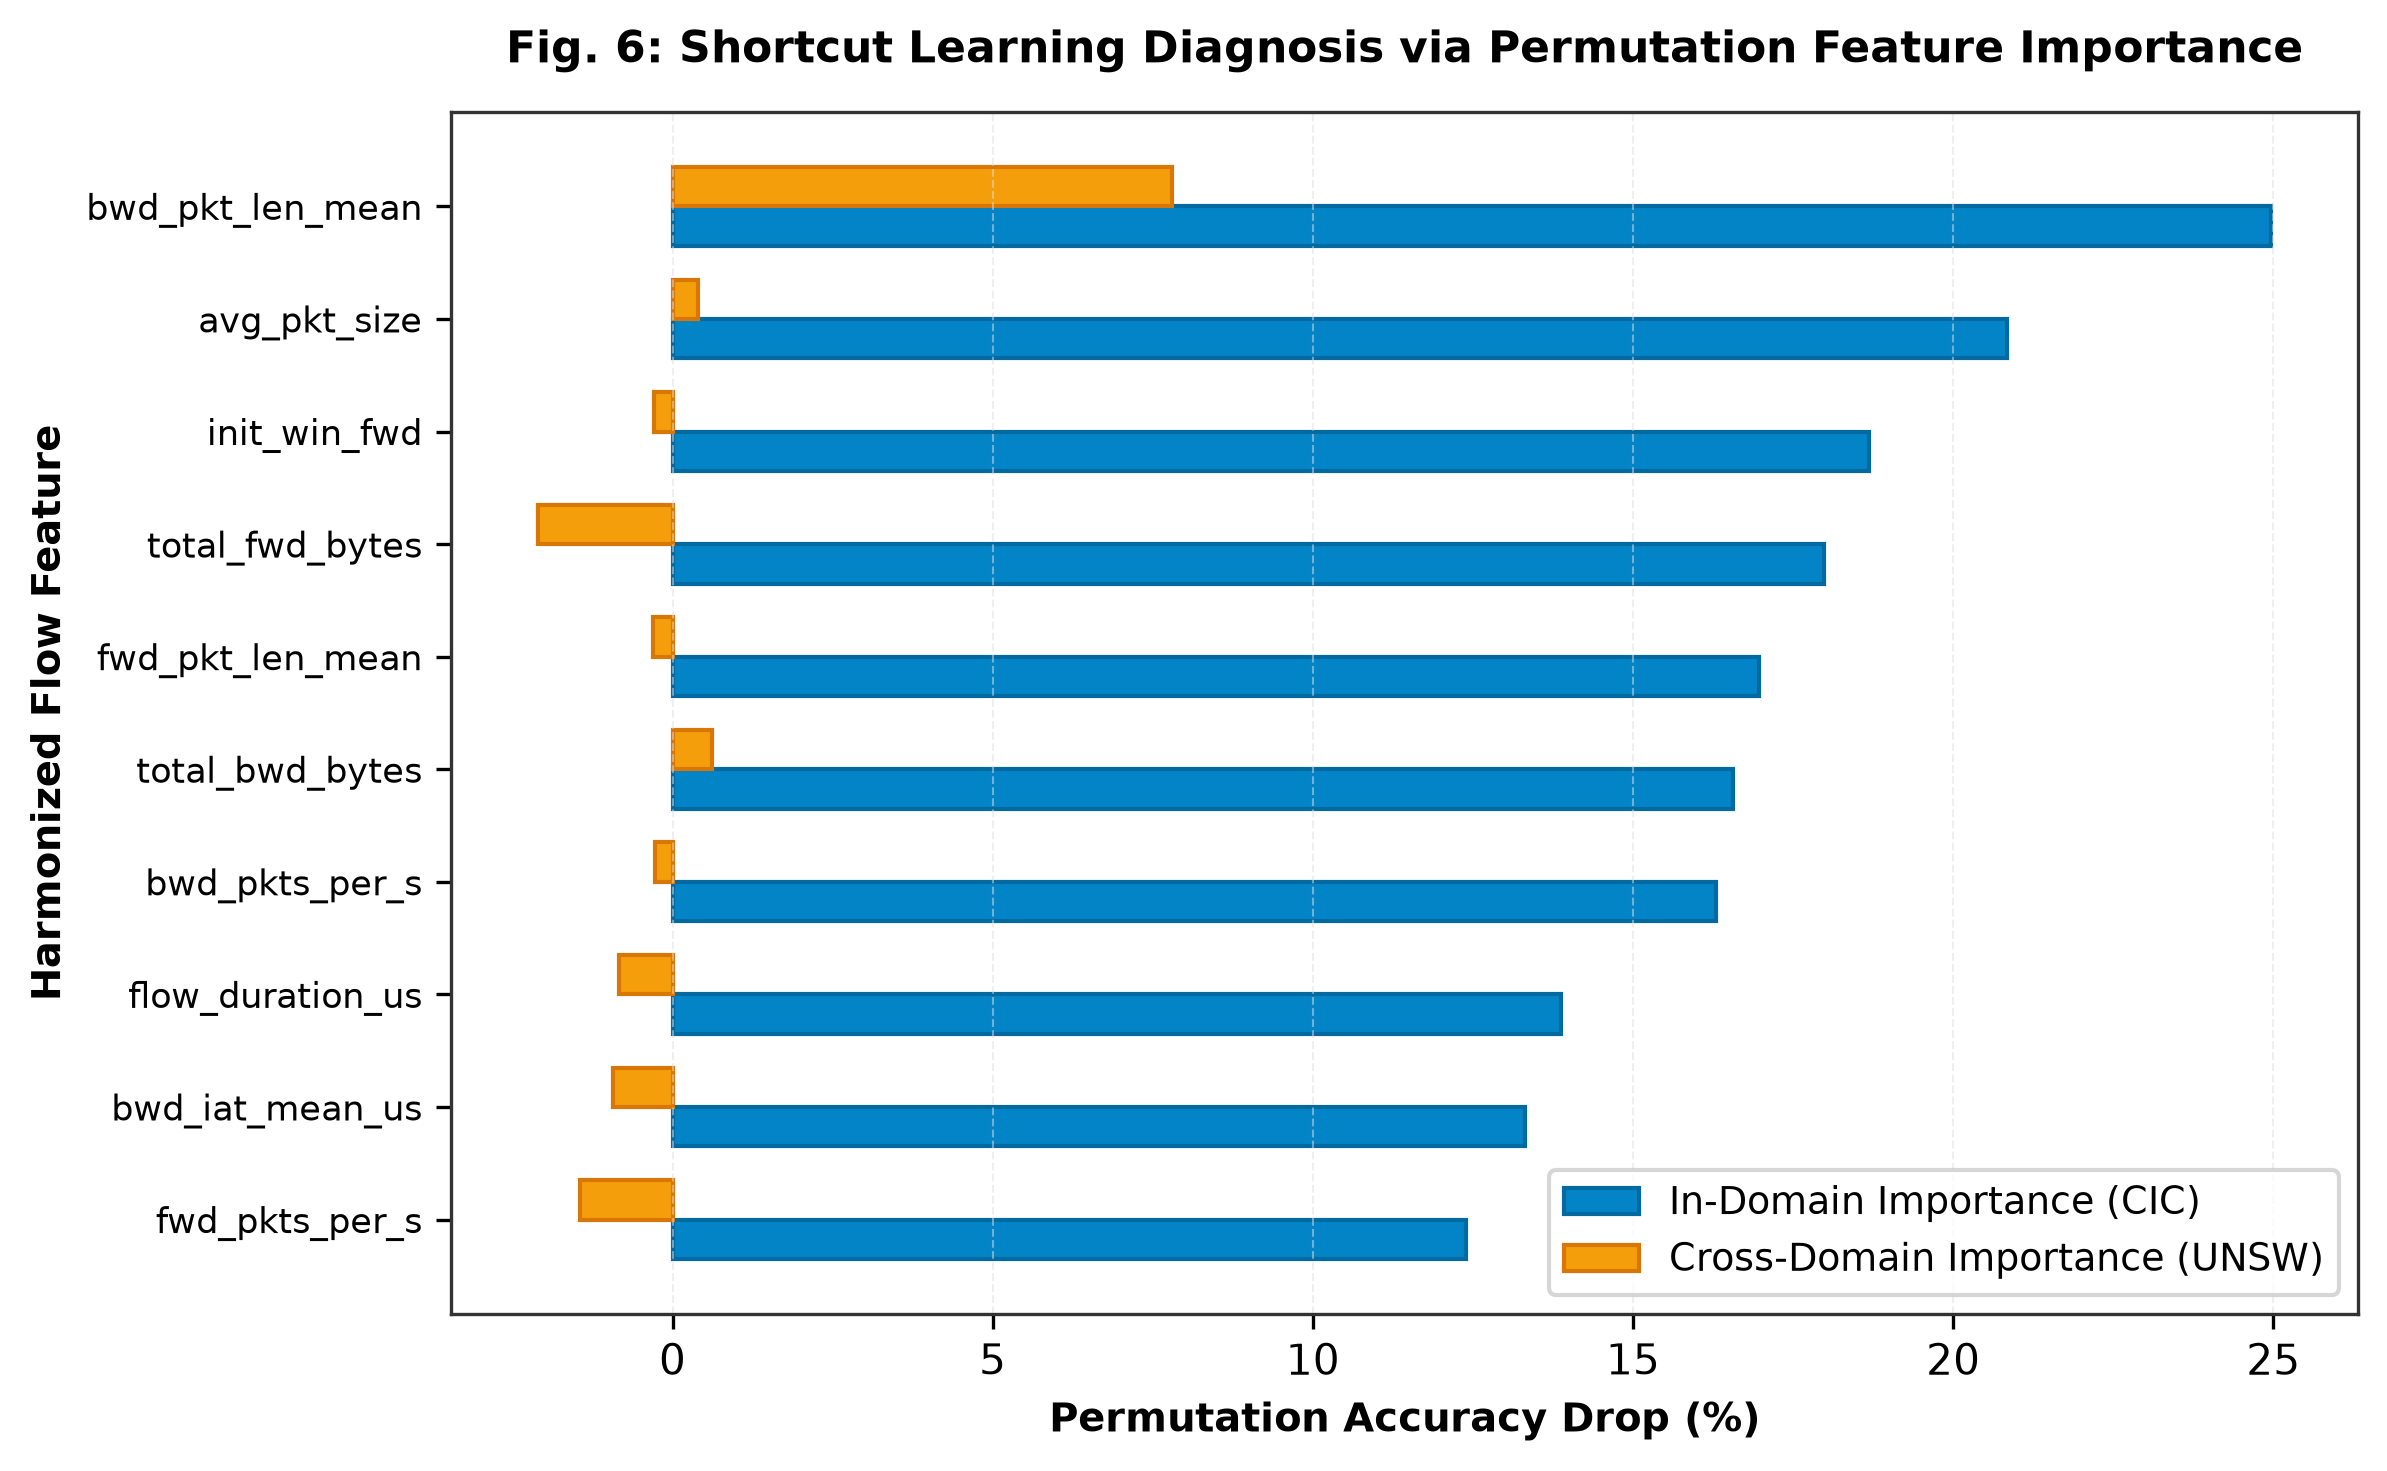
\includegraphics[width=\columnwidth]{figures/fig6_shortcut_importance.png}
\caption{Shortcut Learning Diagnosis via Permutation Feature Importance.}
\label{fig:perm}
\end{figure}

\subsection{Hardware Profiling & Benchmarking}
Table~\ref{tab:benchmarks} and Fig.~\ref{fig:hardware} summarize host CPU execution benchmarks alongside analytical ESP32 edge projections.

\begin{table}[h]
\centering
\caption{Hardware Performance Comparison: Measured Host vs. Analytical ESP32}
\label{tab:benchmarks}
\renewcommand{\arraystretch}{1.1}
\begin{tabular}{llrrr}
\hline
\textbf{Tier} & \textbf{Metric} & \textbf{FP32} & \textbf{INT8} & \textbf{Savings} \\
\hline
Measured on Host & Median Latency & 12.90 $\mu\text{s}$ & 62.70 $\mu\text{s}$ & Host overhead \\
(Intel x86 CPU) & P95 Latency & 14.10 $\mu\text{s}$ & 68.30 $\mu\text{s}$ & Host overhead \\
\hline
Analytical ESP32 & Clock Cycles & 19,920 & \textbf{5,504} & \textbf{-72.37\%} \\
(Xtensa LX6 @ 240MHz) & Projected Latency & 83.00 $\mu\text{s}$ & \textbf{22.93 $\mu\text{s}$} & \textbf{-72.37\%} \\
 & Tensor Arena & 4,304 B & \textbf{4,160 B} & \textbf{-3.35\%} \\
 & Flash Footprint & 4,356 B & \textbf{1,236 B} & \textbf{-71.63\%} \\
 & Energy / Inf & 21.50 $\mu\text{J}$ & \textbf{4.69 $\mu\text{J}$} & \textbf{-78.18\%} \\
 & Active Power & 259.05 mW & \textbf{204.60 mW} & \textbf{-21.02\%} \\
\hline
\end{tabular}
\end{table}

\begin{figure}[t]
\centering
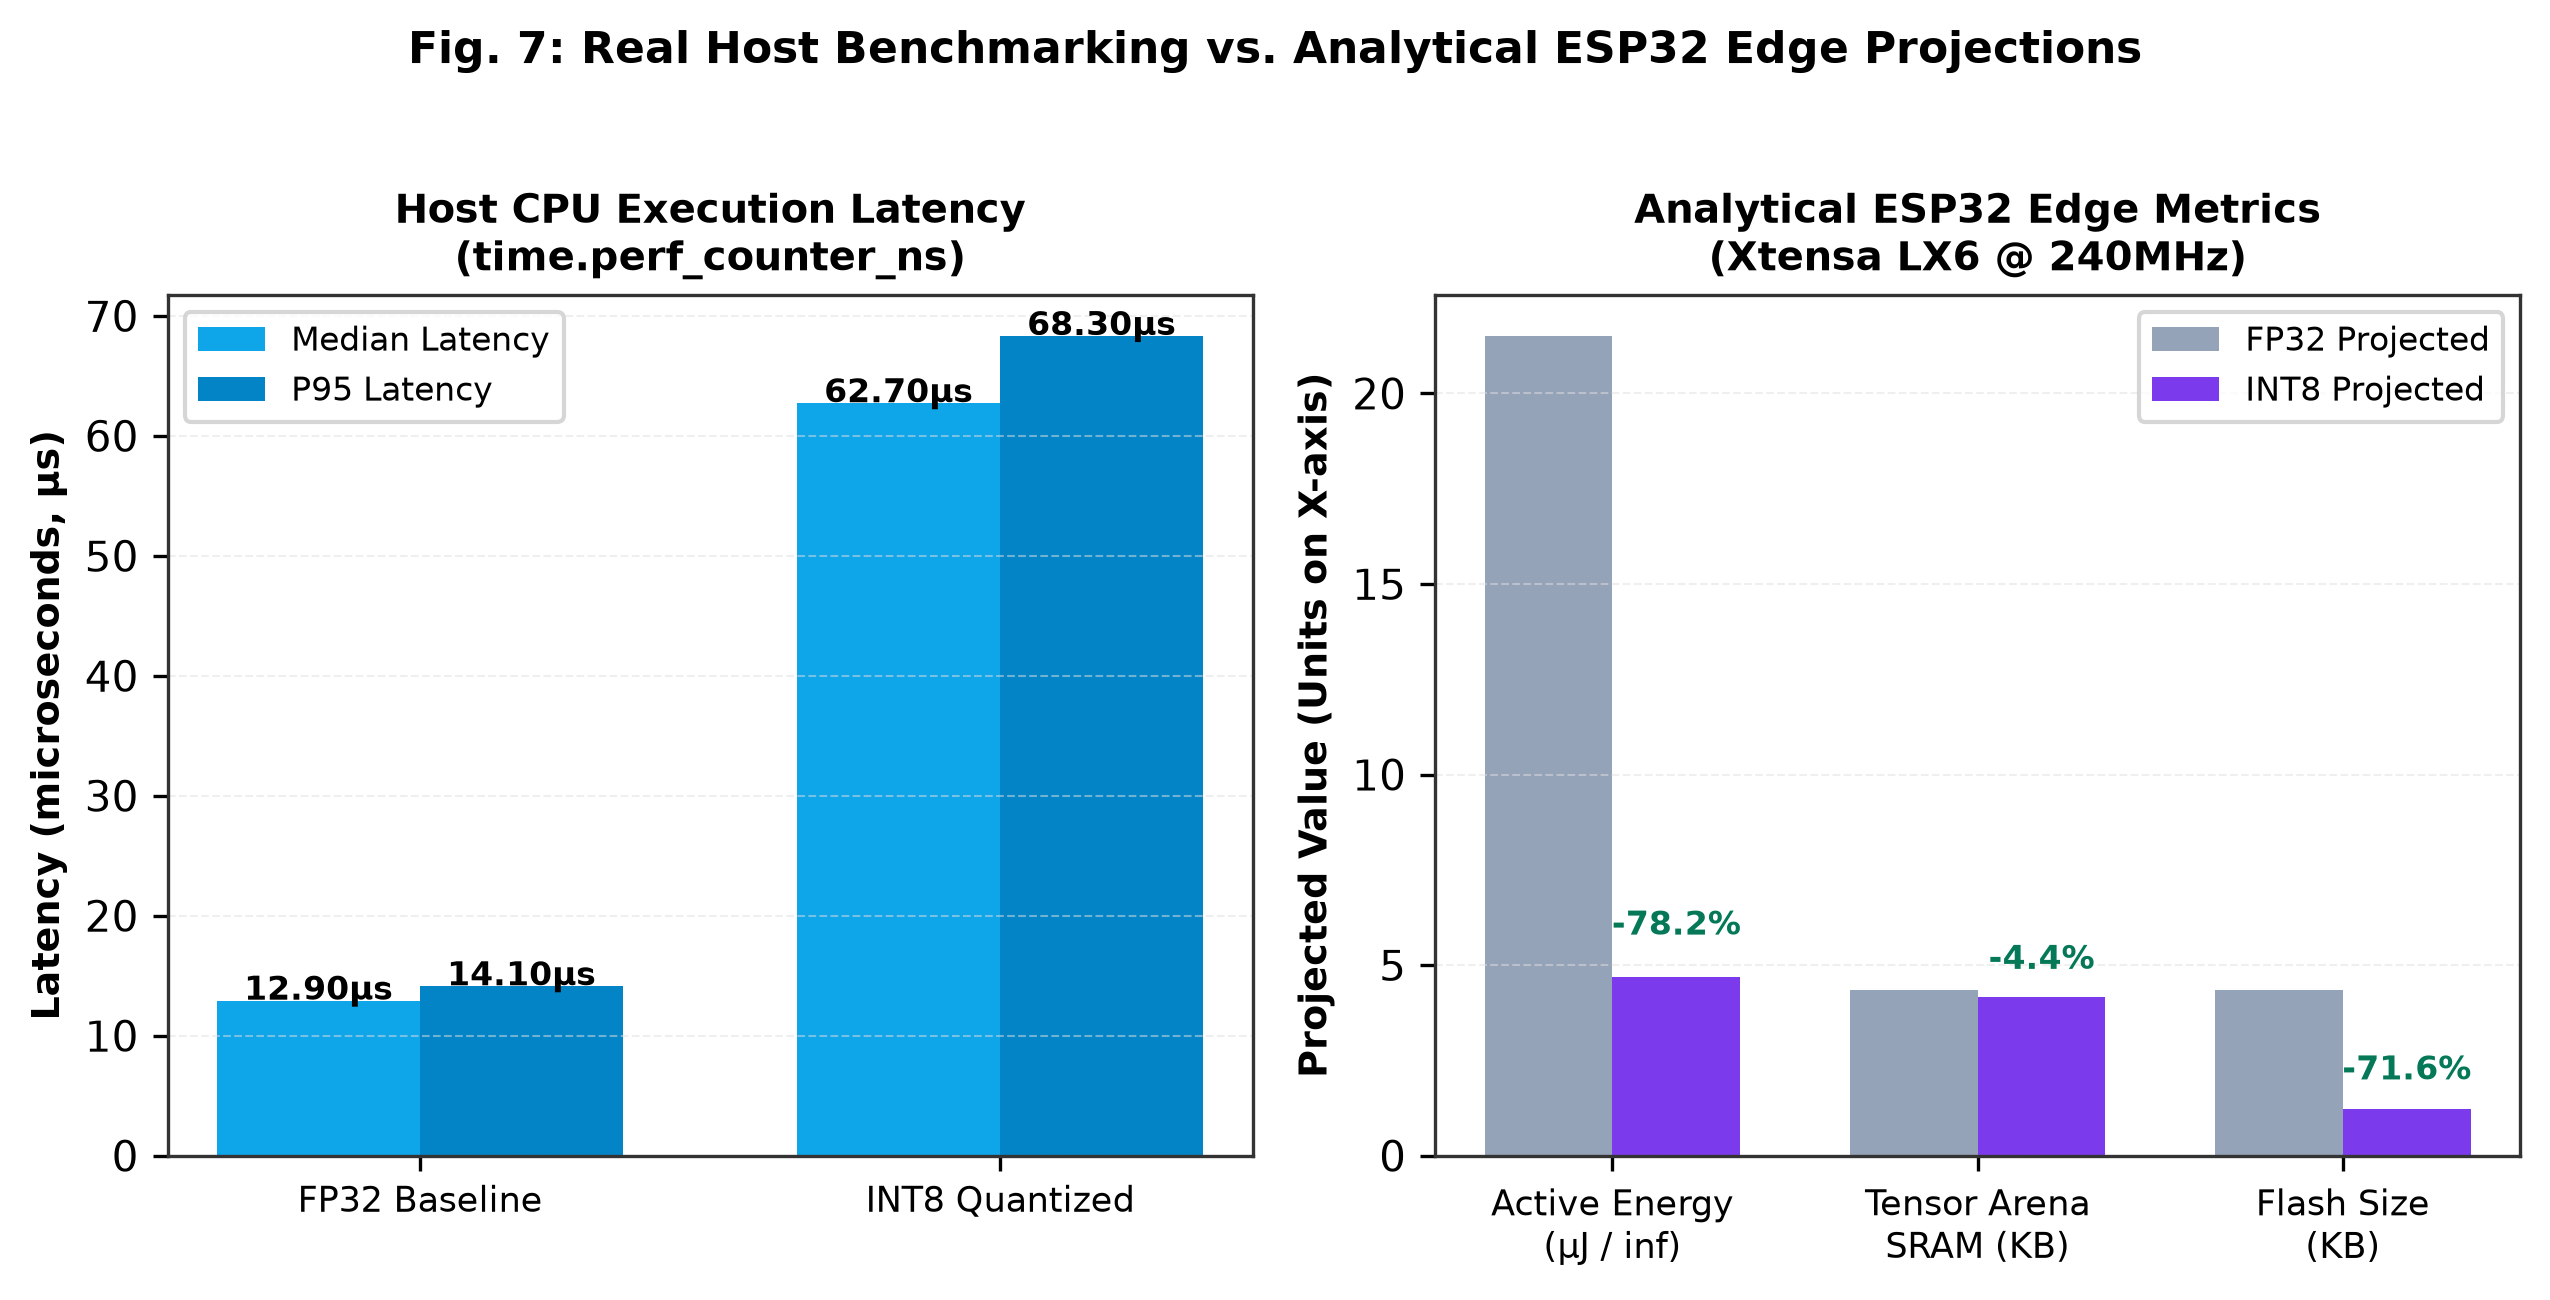
\includegraphics[width=\columnwidth]{figures/fig7_latency_energy_tradeoff.png}
\caption{Real Host Benchmarking vs. Analytical ESP32 Edge Projections.}
\label{fig:hardware}
\end{figure}

On the host x86 workstation, FP32 runs faster ($12.90\ \mu\text{s}$) than INT8 ($62.70\ \mu\text{s}$) due to Python-level integer wrapping overhead and high-throughput AVX2 floating-point vector units. Conversely, on embedded microcontrollers lacking vector floating-point hardware, the analytical model projects an INT8 latency of \textbf{$22.93\ \mu\text{s}$} (a $72.37\%$ speedup over FP32's $83.00\ \mu\text{s}$), requiring only \textbf{$4.69\ \mu\text{J}$ per inference} and slashing flash consumption by \textbf{$71.63\%$}.
